\documentclass{article}

\usepackage[table]{xcolor}
\usepackage[utf8]{inputenc}
\usepackage[style=apa]{biblatex}
\usepackage[margin=1in]{geometry}
\usepackage{hyperref}
\usepackage{indentfirst}
\usepackage{mhchem}
\usepackage{enumitem}
\usepackage{mathtools}
\usepackage{array}
\usepackage{caption}
\usepackage{float}
\usepackage{tabularx}
\usepackage{multirow}
\usepackage{siunitx}
% \usepackage{amsmath}
\usepackage{amssymb}
\usepackage{graphicx}
\usepackage{subcaption}

\addbibresource{references.bib}
\setlength{\bibitemsep}{12pt}
\setlength{\parindent}{0in}
% \setlength{\parskip}{12pt}
\captionsetup[table]{skip=6pt}
\renewcommand{\baselinestretch}{1.15}  % 1.15 spacing

\title{\textbf{The Relationship between Glucose Concentration and the Rate of Carbon Dioxide Production during the Fermentation Process of Yeast}}
\author{}
\date{}

% https://chem-space.com/search
\begin{document}

\pagenumbering{gobble}
\maketitle
\newpage
\pagenumbering{arabic}

\section{Introduction}
I have always enjoyed cooking as a mostly self-taught hobby. Having experimented with multiple aspects of cooking throughout my life eventually led me to explore baking, where I was fascinated by timelapse footages of bread rising in the oven. As such, I was inspired to make my own bread, following basic recipes online with a surface-level understanding of the chemistry involving the release of carbon dioxide from yeast fermentation. However, the realm of baking is very large and not limited to bread only, as there exist many types of doughs for pizza, puff pastry, cookies, etc. One notable difference between these different types of dough is the amount of sugar used, and although some of these repices do not call for yeast, I was still interested by its function in baking, which led me to form my research question: \textbf{``The Relationship between Glucose Concentration and the Rate of Carbon Dioxide Production during the Fermentation Process of Yeast''}.

\section{Background}

\subsection{What Is Yeast}
Yeast are single celled, eukaryotic organisms of the fungus kingdom. Like many living organisms, yeast requires food to survive, namely be converting carbohydrates or sugar sources to energy through either aerobic or anaerobic respiration \parencite{ref}. There exists many types of yeast. The one used in this internal assessment are part of the \emph{Saccharomyces cerevisiae} strain, which can be categorized into brewer's yeast (beer making) and baker's yeast (leavening agent) \parencite{ref}.

\medskip

This internal assessment focuses on the use of active dry yeast, which consists of pellets of live yeast cells coated with a layer of dehydrated cells, \parencite{ref} allowing it to stay dormant to give it a longer shelf life. Hence, active dry yeast must be activated through rehydration in lukewarm water from 37$\,^{\circ}$C to 43$\,^{\circ}$C (optimal fermentation conditions) for 5 to 10 minutes in a process called proofing which also ensures that the yeast is dissolved in the water \parencite{ref}.

\subsection{Aerobic and Anaerobic Respiration in Yeast}
It is well known that yeast reacts with glucose to produce ethanol and carbon dioxide. To understand the details of how this works, it is crucial to understand how yeast undergoes both aerobic and anaerobic respiration.

\medskip

Aerobic respiration is much more efficient and optimal than anaerobic respiration because of the significantly more ATP (adenosine triphosphate, energy carrying molecule) produced. The chemical formula for aerobic respiration is given below:
\begin{equation}
    \ce{\underset{\text{Glucose}}{\ce{C6H12O6}} + 6O2 ->[cellular respiration] 6CO2 + 6H2O + ATP}
\end{equation}

Going into the details of aerobic respiration its three steps:
\begin{enumerate}[topsep=\parskip, noitemsep]
    \item Glycolysis
    \item Tricarboxylic acid cycle
    \item Oxidative phosphorylation (where most of the APT is produced)
\end{enumerate}

% TODO italicize key terms?

\medskip

However, the focus of this internal assessment is on anaerobic respiration of yeast because the amount of oxygen was limited given the environment that the experiment was carried out in. The only similarity between aerobic and anaerobic respiration is glycolysis, which prompts to explore this step in more detail \parencite{ref}.

\medskip

The first step of glycolysis converts glucose into fructose 1,6-biphosphate (F-1,6-BP), outlined in the figure below:
\begin{figure}[H]
    \centering
    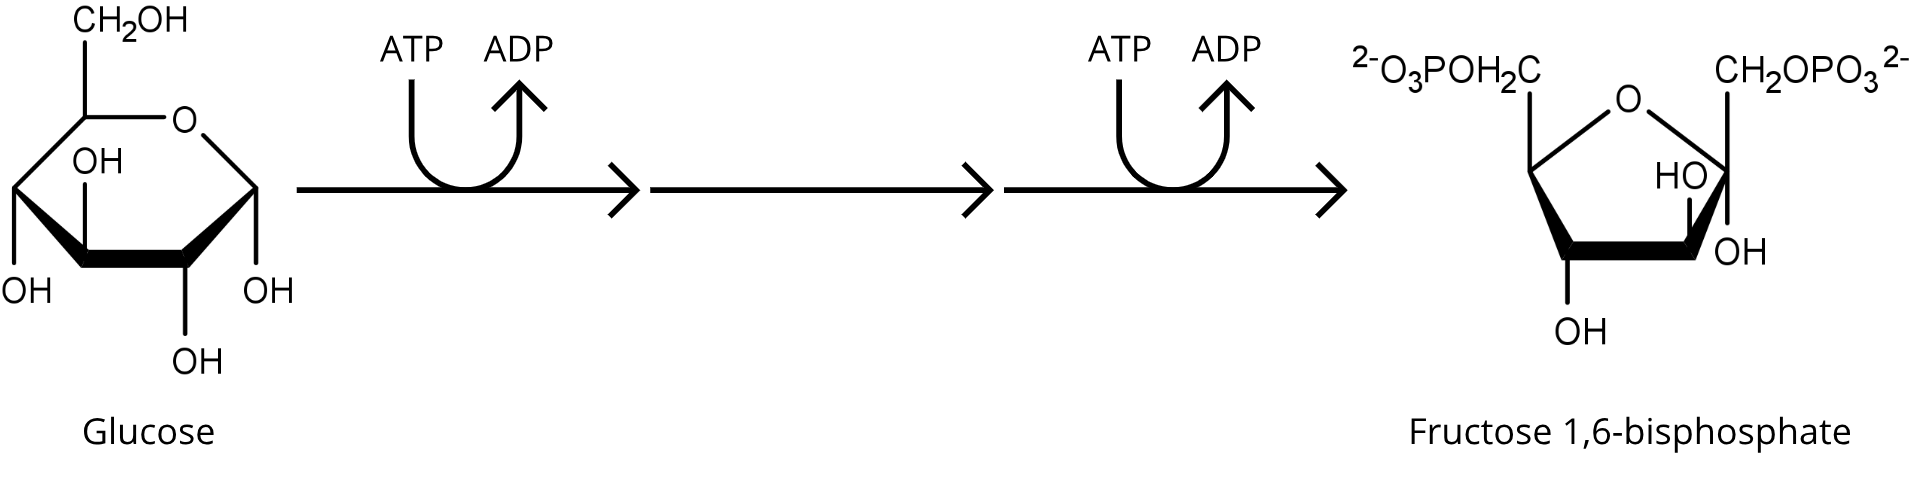
\includegraphics[width=0.8\linewidth]{figures/figure_01.png}
    \caption{Conversion of glucose to F-1,6-BP. Intermediate steps are represented by the arrows.}
    \label{fig:figure1}
\end{figure}

Glucose goes through a series of reactions catalyzed by multiple enzymes, which consumes 2 ATP in the process. ATP turns to ADP (adenosine diphosphate) when a phosphate group (\ce{HPO_{4}^{2-}}) gets transferred from the ATP to the sugars that glucose gets broken down into, eventually leading to the formation of F-1,6-BP.

\medskip

The second step of glycolysis involves splitting F-1,6-BP into 2 three-carbon fragments, glyceraldehyde 3-phosphate (GAP) and dihydroxyacetone phosphate (DHAP), outlined in the figure below:
\begin{figure}[H]
    \centering
    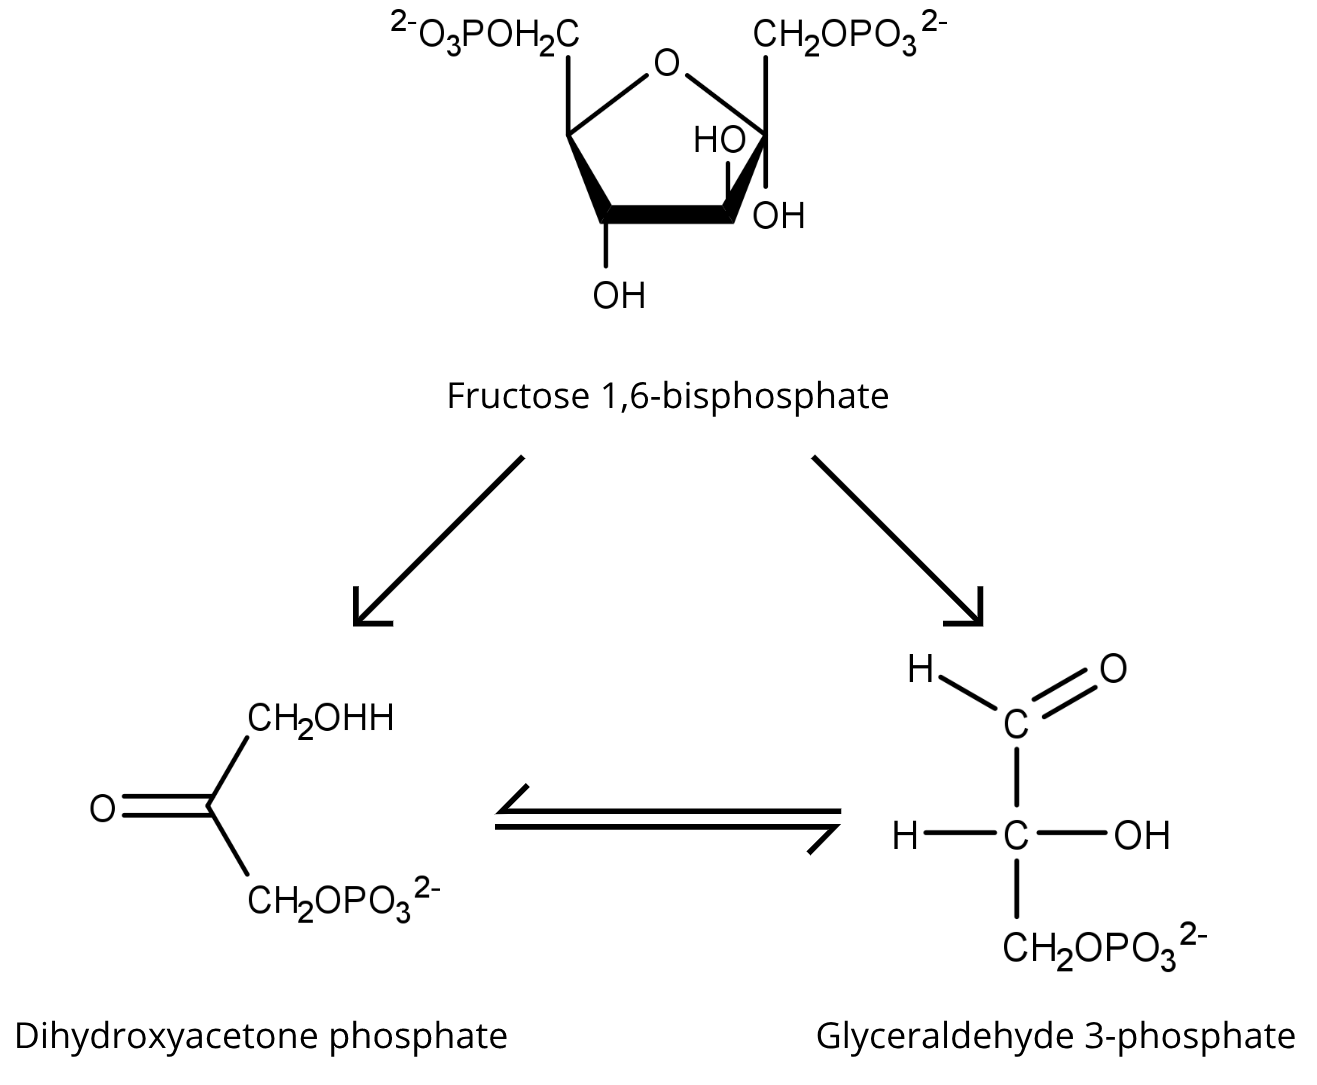
\includegraphics[width=0.55\linewidth]{figures/figure_02.png}
    \caption{Conversion of F-1,6-BP to GAP and DHAP}
    \label{fig:figure1}
\end{figure}

\medskip

When catalyzed with an enzyme, F-1,6-BP splits into the three-carbon fragments but only GAP can continue the glycolysis process. However, GAP and DHAP exist in equilibrium, meaning all the DHAP eventually turns to GAP.

\medskip

The third and final step of glycolysis converts the DHAP to pyruvate, another three-carbon molecule while producing ATP, outlined in the figure below:
\begin{figure}[H]
    \centering
    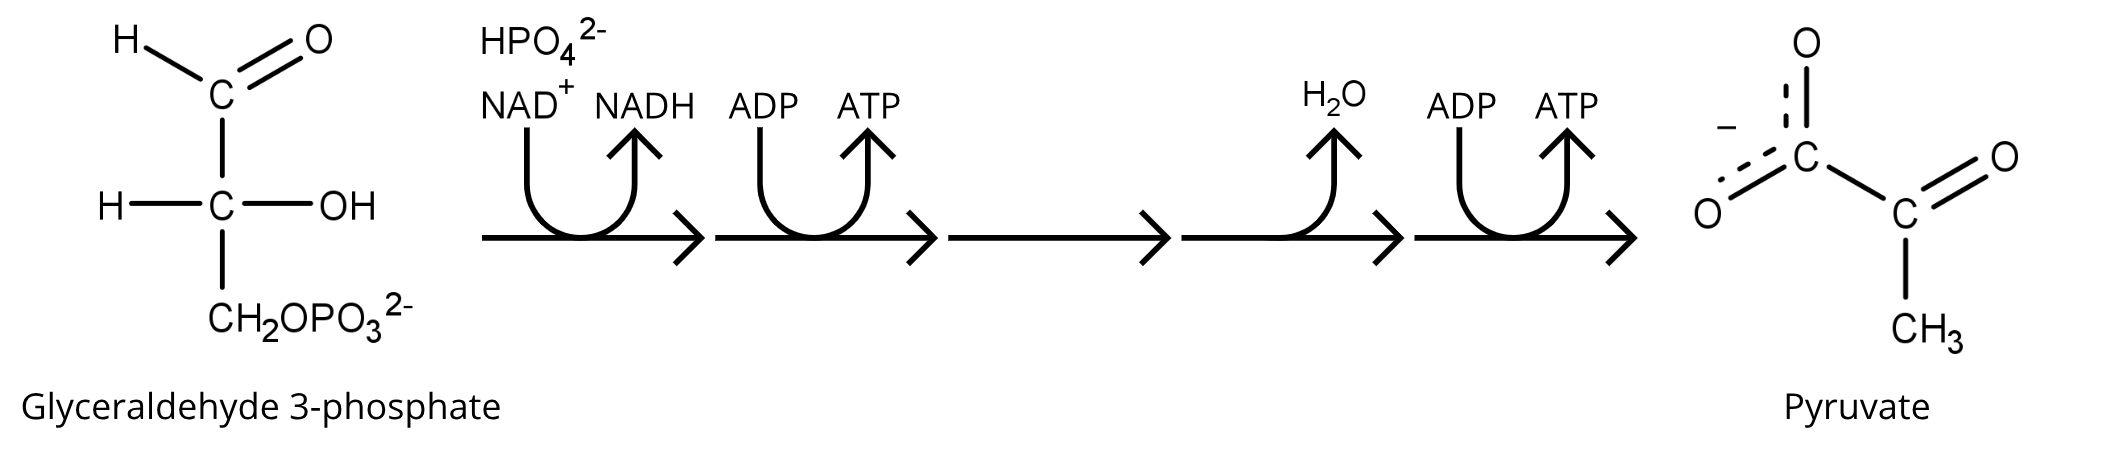
\includegraphics[width=0.886\linewidth]{figures/figure_03.png}
    \caption{Conversion of DHAP to pyruvate. Intermediate steps are represented by the arrows.}
    \label{fig:figure1}
\end{figure}

\medskip

Like glucose, GAP goes through another series of reactions catalyzed by multiple enzymes that eventually turn it into Pyruvate. During one step of the process, a molecule called \ce{NAD+} (nicotinamide adenine dinucleotide, a coenzyme found in the cell that is crucial to metabolic processes) \parencite{ref} gets reduced to NADH wihle GAP is simultaneously oxidized. The phosphate groups that were given from the ATP in the first step is combined with ADP twice to form 2 ATP. Since the DHAP got converted into GAP in the previous step, 4 total ATP is formed \parencite{ref}.

\medskip

The net equation for the formation of pyruvate is thus given by:
\begin{equation}
    \ce{Glucose + 2HPO_{4}^{2-} + 2ADP + 2NAD+ -> 2Pyruvate + 2ATP + 2 NADH + 2H+ + 2H2O}
\end{equation} % TODO \ce{2pyruvate} issue
According to Equation (2), the end result of glycolysis leaves 2 pyruvate, 2 NADH, 2 ATP, 2 \ce{H2O}, and 2 \ce{H+}. If there is unreacted glucose, glycolysis will continue. However, a cell's supply of \ce{NAD+} is limited, so it must be regenerated. In aerobic respiration, the pyruvate goes through the tricarboxylic acid cycle to produce even more NADH that eventually gets oxidized to \ce{NAD+} during oxidative phosphorylation, which produces most of the ATP associated with aerobic respiration as a bonus. In anaerobic respiration, fermentation provides an alternate pathway to turn the NADH back to \ce{NAD+}.

\medskip

% TODO figure out when to use name and chemical
% TODO chemical capitals
% TODO add more references
For yeast,  alcoholic fermentation converts pyruvate into ethanol and carbon dioxide, both of with are waste products. It consists of two steps that are also catalyzed by enzymes. The first step in this conversion process involves the decarboxylation of pyruvate to acetaldehyde, producing carbon dioxide as a by product, as shown below:
\begin{equation}
    \ce{\underset{\text{Pyruvate}}{\ce{CH3COCOO-}} + H+ -> \underset{\text{Acetaldehyde}}{\ce{CH3CHO}} + CO2}
\end{equation}

In the second step, acetaldehyde gets reduced to ethanol and NADH gets oxidized to \ce{NAD+}, effectively regenerating \ce{NAD+} to be reused in glycolysis:
\begin{equation}
    \ce{CH3CHO + NADH + H+ -> \underset{\text{Ethanol}}{\ce{C2H5OH}} + NAD}
\end{equation}

Equation (3) can be substituted in Equation (2) after some rearranging:
\begin{equation*}
    \ce{Glucose + 2HPO_{4}^{2-} + 2ADP + 2NAD+ -> \textcolor{red}{\ce{2CH3CHO}} + \textcolor{red}{\ce{2CO2}} + 2ATP + 2NADH + 2H2O}
\end{equation*}

Adding \ce{2H+} on both sides and substituting Equation (4)
\begin{equation*}
    \ce{Glucose + 2HPO_{4}^{2-} + 2ADP + 2NAD+ + \textcolor{blue}{\ce{2H+}} -> \textcolor{blue}{\ce{2C2H5OH}} + \textcolor{blue}{\ce{2NAD+}} + 2ATP + 2H2O}
\end{equation*}

Cancelling \ce{2NAD+} on both sides gives:
\begin{equation}
    \ce{C6H12O6 + 2HPO_{4}^{2-} + 2ADP + 2H+ -> 2C2H5OH + 2CO2 + 2ATP + 2H2O}
\end{equation}

Which is more familiarly known as:
\begin{equation}
    \ce{C6H12O6 ->[yeast] 2C2H5OH + 2CO2}
\end{equation}

\section{Kinetics}  % TODO fermentation process changen to alcoholic fermentation

\subsection{Basic Kinetics}
Given the following chemical reaction denoting alcoholic fermentation:
\begin{equation}
    \ce{A -> 2B + 2C}
\end{equation}
Studying the kinetics of this reaction is useful for performing further levels of analysis. Kinetics in chemistry refers to the study of rates of chemical reactions, which is a measurement of the change in concentration of products and reactants over a period of time \parencite{ref}.

\medskip

The rate of reaction, also known as the reaction velocity $V$ with respect to a compound within the chemical equation is represented as the change in concentration of that compound over the change in time multiplied by the inverse of its stoichiometric coefficient:
\begin{equation}
    V = \text{rate} = -\frac{d[A]}{dt} = \frac{1}{2}\frac{d[B]}{dt} = \frac{1}{2}\frac{d[C]}{dt}
\end{equation}

Additionally, the rate law states how the reaction velocity will be directly proportional to the product of reactants, each reactant raised to a power:
\begin{equation}
    V = k[A]^m
\end{equation}
where $k$ is is the rate constant \parencite{ref} and the sum of the powers denote the order of the reaction. In the case of alcoholic fermentation, the order is purely dependent on $m$.

\medskip

If the order of the reaction is 0, the rate of reaction will not be dependent on the concentration of the reactants, that is $V = k[A]^0 = k$. If the order of the reaction is 1, the rate of reaction will be proportional to the concentration of the reactants, that is $V = k[A]^1 = k[A]$.

\subsection{Michaelis Menten Enzyme Kinetics}
When reactions are enzyme-catalyzed, enzyme kinetics proves to be a better model at predicting the behvaiour of the reaction. The Michaelis Menten model, proposed by Leonor Michaelis and Maud Menten in 1913 is concerned with $V_0$, the relationship between initial reaction velocity (rate of enzyme catalysis) and the substrate concentration:
\begin{equation}
    \ce{E + S <=>[k_1][k_{-1}] ES ->[k_2] E + P}
\end{equation}

Where
\begin{itemize}[topsep=\parskip, noitemsep]
    \item E denotes the enzyme, which is treated as zyamze, the enzyme responsible for fermentation in yeast
    \item S denotes the substrate, the glucose solution
    \item P denotes the product, the carbon dioxide gas formed
    \item ES denotes the enzyme substrate complex, an intermediate step in where the enzyme temporarily binds to the substrate, which eventually gets dissociated into the same enzyme and the product
\end{itemize}

\medskip

Additionally:
\begin{itemize}[topsep=\parskip, noitemsep]
    \item $k_1$ denotes the rate constant associated with the formation of \ce{ES}
    \item $k_{-1}$ is associated with the breakdown of \ce{ES} to \ce{E}
    \item $k_2$ is associated with the dissociation of \ce{ES} to \ce{E + P}
\end{itemize}

\medskip

Technically, $k_{-2}$ also exists, but since the Michaelis Menten model is only concerned with $V_0$ so the breakdown of \ce{E + P} into \ce{ES} is negligible.

\medskip

Firstly, a formula can be derived for $V_0$, using the equation \ce{ES -> E + P}:
\begin{equation}
    V_0 = k_2 [\ce{EP}]
\end{equation}

The rate of formation of \ce{ES} is given by:
\begin{equation}
    k_1 [\ce{E}]
\end{equation}

And the rate of breakdown of \ce{ES} is given by:
\begin{equation}
    (k_{-1} + k_2) [\ce{ES}]
\end{equation}

In 1924, George Briggs and John Haldane proposed the steady state assumption to further simplify enzyme kinetics, which assumes that the rate of formation is equal to the rate of breakdown of \ce{ES}:
\begin{equation}
    k_1 [\ce{E}] = (k_{-1} + k_2) [\ce{ES}]
\end{equation}

Rearranging Equation (14) gives:
\begin{equation}
    \frac{[\ce{E}][\ce{S}]}{[\ce{ES}]} = \frac{k_{-1}+k_2}{k_1}
\end{equation}

$\frac{k_{-1}+k_2}{k_1}$ can be defined as a new variable $K_m$, the Michaelis constant. Additionally, the equation can be rearranged to represent [\ce{ES}] in terms of concentrations of known substances:
\begin{equation}
    [\ce{ES}] = \frac{[\ce{E}][\ce{S}]}{K_m}
\end{equation}

Considering the total amount of enzyme in the reaction as $\ce{E_T}$, which consists of enzymes bounded to the substrate and free enzymes. [\ce{E_T}] can then be represented as follows:
\begin{equation}
    [\ce{E_T}] = [\ce{E}] + [\ce{ES}]
\end{equation}

Solving Equation (17) for [\ce{E}] and substituting it in Equation (16) gives:
\begin{equation}
    [\ce{ES}] = \frac{([\ce{E_T}] + [\ce{ES}]) [\ce{S}]}{K_m}
\end{equation}

Equation (18) is rearranged to represent [\ce{ES}] in terms of known values:
\begin{equation}
    [\ce{ES}] = [\ce{E_T}]\frac{[\ce{S}]}{\ce{S} + K_m}
\end{equation}

Taking Equation (11) and substituting [\ce{ES}]:
\begin{equation}
    V_0 = k_2[\ce{E_T}]\frac{[\ce{S}]}{\ce{S} + K_m}
\end{equation}

$k_2[\ce{E_T}]$ can also be used to describe the reaction velocity. If [\ce{E_t}] was used in place of [\ce{ES}] in Equation (11), all enzymes are undergoing catalysis. This is defined as $V_{max}$, the maximum reaction velocity for a set of conditions. Rewriting Equation (20) gives the final Michaelis Menten equation:
\begin{equation}
    V_0 = V_{max}\frac{[S]}{[S] + K_m}
\end{equation}

If $[\ce{S}] << K_m$, then $V_0 \approx V_{max}\frac{[\ce{S}]}{K_m}$, meaning that the reaction velocity will be directly proportional to the substrate concentration (first order reaction). If $[\ce{S}] >> K_m$, then $V_0 \approx V_{max}$, meaning the reaction velocity does not depend on the substrate concentration (zero order reaction). If $[\ce{S}] = K_m$, then $V_0 = \frac{V_{max}}{2}$, meaning $K_m$ equals the substrate concentration at half the maximum reaction velocity. This information makes intuitive sense when graphed:

\section{Design}

\newpage

\subsection{Safety}
Before starting the lab, physical, environmental, and ethical safety issues must be taken into account. The following table lists them out:
\begin{table}[H]
\centering
\caption{Safety hazards and their considerations}
\label{table:1}
\begin{tabularx}{\textwidth} {
    | >{\hsize=.4\hsize \linewidth=\hsize \raggedright\arraybackslash}X
    | >{\hsize=.6\hsize \linewidth=\hsize \raggedright\arraybackslash}X |
}
    \hline
    \rowcolor[HTML]{CCCCCC} Hazard & Safety Considerations \\
    \hline
    Risk of broken glassware & If possible, glassware should be handled with both hands to minimize the chance of breakage. Extra care should be taken during the cleaning process as glassware may be slippery when wet.\\
    \hline
    Risk of hotplate burns & It is important to not touch the hotplate, even when it's off. Once finished using, the hotplate and any lab apparatus that was on it should be cooled before storage.\\
    \hline
    Wiring and electronics & Baggy clothing should not be worn due to the risk of accidentally tangling with wires. If not used in an experiment, chemicals should be kept a far distance from electronics.\\
    \hline
    Dumping products down the drain & Yeast should not be dumped down the drain unless it is dissolved and heavily diluted. Similarly, dumping concentrated ethanol is hazardous unless heavily diluted as well. \parencite{ref}\\
    \hline
    Wasting yeast & Yeast is used in baking and wasting it can be an ethical concern. Any unused yeast that hasn't been contaminated with a scoopula should be returned.\\
    \hline
    Spills and splashes & Goggles should be worn until the lab has been cleared up to prevent chemicals from coming in contact with the eyes. Paper towels should be kept handy at all times to clean up spills.\\
    \hline
\end{tabularx}
\end{table}

\subsection{Hypothesis}
After the yeast is fully activated and dissolved and mixed with glucose, the concentration of carbon dioxide produced will increase linearly for a short time until tapering off as all of the glucose gets used when the reaction goes to completion. For lower concentrations of glucose, the initial reaction velocity and the final concentration of carbon dioxide gas produced will be smaller than higher concentrations of glucose. When plotting the initial reaction velocity against the concentration of glucose, the curve of best-fit will fit the Michaelis-Menten kinetics model, passing through the origin.

% todo table below or following table
\subsection{Variables}
The following table lists out all dependent, independent, and control variables used in my experiment, along with reasons and details to why each variable was chosen to be a specific type:
\begin{table}[H]
\centering
\caption{Variables used in my experiment}
\label{table:2}
\begin{tabularx}{\textwidth} {
    | >{\hsize=.2\hsize \linewidth=\hsize \raggedright\arraybackslash}X
    | >{\hsize=.3\hsize \linewidth=\hsize \raggedright\arraybackslash}X
    | >{\hsize=.5\hsize \linewidth=\hsize \raggedright\arraybackslash}X |}
    \hline
    \rowcolor[HTML]{CCCCCC} Variable type & Description & Reason and details \\
    \hline
    \multirow[t]{2}{\hsize}{Independent} & Time (\si{s}) & Time is an independent variable when plotting a concentration-time graph \\
    \cline{2-3}
    % TODO units same font as latex text issue
    % TODO more consistent use of \si for all units
    & Glucose concentration (\si{ppm}) & The glucose concentration will be varied by modifying the mass of glucose. Specific units for ppm are \si{mg.L^{-1}}. \\
    \hline
    \multirow[t]{2}{\hsize}{Dependent} & Carbon dioxide concentration (\si{ppm}) & When the reaction occurs, the carbon dioxide concentration will vary with time. Specific units for ppm are \si{mL.L^{-1}}. \\
    \cline{2-3}
    & Initial rate of carbon dioxide production (\si{ppm.s^{-1}}) & The initial rate of carbon dioxide production will depend on the glucose concentration. \\
    \hline
    \multirow[t]{3}{\hsize}{Control} & Volume of deionized water (\si{mL}) & Deionized water will be used instead of tap water since ions in tap water may influence rate of reaction. \\
    \cline{2-3}
    & Temperature of water (\si{\celsius}) and mass of yeast used (\si{g}) & These variables will be kept constant because they both influence the rate of carbon dioxide production and the effects of only one independent variable is studied. \\
    \cline{2-3}
    & Time for the yeast to fully dissolve and activate & The yeast is given ample time to dissolve and activate in the deionized water. If the glucose is added too early, then the initial rate of reaction will be smaller than expected. \\
    \hline
\end{tabularx}
\end{table}

\subsection{Apparatus and Experimental Setup}
The following materials were used in my experiment:
\begin{table}[H]
\centering
\caption{Categorized materials list}
\label{table:3}
\begin{tabularx}{\textwidth} {
    | >{\hsize=.35\hsize \linewidth=\hsize \raggedright\arraybackslash}X
    | >{\hsize=.65\hsize \linewidth=\hsize \raggedright\arraybackslash}X |}
    \hline
    \rowcolor[HTML]{CCCCCC} Category & Materials \\
    Compounds and reactants & \textbullet Red Star active dry yeast \\
    & \textbullet Lab grade glucose \\
    & \textbullet Deionized water \\
    \hline
    Containers and tools & \textbullet 1\,\si{L} beaker \\
    & \textbullet 100\,\si{mL} graduated cylinder $(\pm0.5\,\si{cm})$ \\  % TODO turn brackets into $()$
    & \textbullet 250\,\si{mL} Nalgene bottle \\
    & \textbullet Magnetic stir bar \\
    & \textbullet Folded paper for holding reactants \\
    & \textbullet Scoopula \\
    \hline
    Devices & \textbullet Barnstead/Thermolyne magnetic stirring hotplate \\
    & \textbullet Vernier LabQuest2 \\
    & \textbullet Vernier stainless steel temperature probe \\
    & \textbullet A\&D EJ-200 scale $(\pm0.005\,\si{cm})$ \\
    & \textbullet Vernier \ce{CO2} gas sensor $(\pm0.005\,\si{cm})$ \\
    \hline
\end{tabularx}
\end{table}

The experiment was carried out following the procedure below:
\begin{enumerate}[topsep=\parskip, noitemsep]
    % \setlength\itemsep{-5pt}
    \item Approximately 0.5\,\si{L} of deionized water was prepared in a 1\,\si{L} beaker and placed on a magnetic stirring hotplate.
    \item The Vernier LabQuest was plugged in with a Vernier temperature probe.
    \item THe water was heated until it reached approximately 37\,\si{\celsius}. The temperature of the hotplate was kept at around 40\,\si{\celsius} to 45\,\si{\celsius} to account for cooling.
    \item 0.1\,\si{g} of glucose and 2\,\si{g} of Red Star active dry yeast were weighed
    \item The yeast was deposited in the 250\,\si{ml} Nalgene bottle with the magnetic stir bar.
    \item 100\,\si{ml} of water measured with a graduated cylinder was poured from the 1\,\si{L} beaker to the Nalgene bottle.
    \item The bottle was transferred to the warm water bath with its cap was screwed on.
    \item The \ce{CO2} gas sensor was connected and calibrated to read high concentrations of \ce{CO2} gas. The LabQuest was set to 20 seconds per sample for 10 minutes.
    \item Magnetic stirring was activated to mix the yeast solution to ensure that all the yeast was dissolved and activated. During this phase, observations were recorded and the \ce{CO2} gas sensor was warmed up to read a baseline concentration.
    \item After the yeast was activated glucose was deposited in the bottle and the \ce{CO2} gas sensor was immediately swapped with the cap to block \ce{CO2} from escaping.
    \item The Nalgene-\ce{CO2} sensor setup was lightly swirled around the beaker to allow the stir bar to reach all corners of the bottle.
    \item After 10 minutes of fermentation, data was exported to a USB and the \ce{CO2} gas sensor was removed. Observations were made as the reaction took place.
    \item The \ce{CO2} gas sensor was wiped to remove condensation and fanned to remove residual \ce{CO2}. The Nalgene bottle was thoroughly rinsed and fanned to remove any yeast-glucose solution and residual \ce{CO2} gas.
    \item THe 1\,\si{L} beaker was filled with more distilled water if there was not enough to half-submerge the Nalgene bottle.
    \item Steps 3 to 14 were repeated until 2 trials of data were collected for 0.1\,\si{g}, 0.25\,\si{g}, 0.5\,\si{g}, and 1\,\si{g} of glucose.
\end{enumerate}

\section{Data Collection and Processing}
Listed below are general qualitative observations that were common with all trials:
\begin{itemize}[topsep=\parskip, noitemsep]
    \item When the yeast was all dissolved, the solution turned into a consistency similar to oat-milk, light brownish colour
    \item The glucose dissolves very quickly when stirred
    \item When the solution was dumped after each trial, a smell of ethanol was noted
\end{itemize}

\medskip

The following table displays qualitative observations that were observed for different masses of glucose added. A corresponding concentration is calculated for each mass:
\begin{table}[H]
\centering
\caption{Observations and concentrations for different masses of glucose added}
\label{table:4}
\begin{tabularx}{\textwidth} {
    | >{\hsize=.3\hsize \linewidth=\hsize \raggedright\arraybackslash}X
    | >{\hsize=.3\hsize \linewidth=\hsize \raggedright\arraybackslash}X
    | >{\hsize=.4\hsize \linewidth=\hsize \raggedright\arraybackslash}X |}
    \hline
    \rowcolor[HTML]{CCCCCC} Mass /\ce{g} $\pm0.01\,\si{g}$ & Concentration /\si{M} & Observations \\
    \hline
    0.10 & $0.0056 \pm 0.0006$ & Enough condensation to cover top of bottle, solution was very consistent and smooth \\
    \hline
    0.25 & $0.0139 \pm 0.0006$ & A lot of condensation, considerably more than 0.1\,\si{g}, some condensation started to drip back into the solution \\
    \hline
    0.50 & $0.0278 \pm 0.0007$ & When mixing solution, some white foam appeared on top, a good amount of condensation was formed \\
    \hline
    1.00 & $0.0555 \pm 0.0008$ & Less condensation was observed than smaller concentrations, traces of very fine precipitate left at the bottom, depsite stirring with a stir bar \\
    \hline
\end{tabularx}
\end{table}

A sample calculation for the concentration uncertainty using the basic method is provided below for mass 0.5\,\si{g}. The molar mass of glucose is taken to be 180.18\,\si{g.mol^{-1}} \parencite{ref}:
\begin{align*}
    c &= \frac{n}{v} = \frac{m/M}{v} \\
    &= \frac{0.5/180.18}{0.1} = 0.02775\,\si{mol.L^{-1}} \\  %% TODO better equations
    \Delta c &= c\left(\frac{\Delta m}{m} + \frac{\Delta v}{v}\right) = 0.02775\left(\frac{0.01}{0.5} + \frac{0.0005}{0.1}\right) \\
    &= 0.000694\,\si{mol.L^{-1}} \\
    \therefore\,c &= (0.0278 \pm 0.0007)\,\si{mol.L^{-1}}
\end{align*}

%% TODO reaction velocity vs rate of reaction
The raw data collected were concentration-time graphs generated by the Vernier \ce{CO2} gas sensor. In total, 2 sets of data were collected for each concentration. As an example, the first tria for 0.5\,\si{g} of glucose added is shown below. The initial reaction velocity was taken to be the slope of the line of best fit for the whole scatter plot because the reaction has not reached equilibrium. A full list of graphs and raw data can be found in the appendix.  %% TODO specify which appendix, full "list" -> "list" not the right word to use
\begin{figure}[H]
    \renewcommand{\figurename}{Graph}
    \centering
    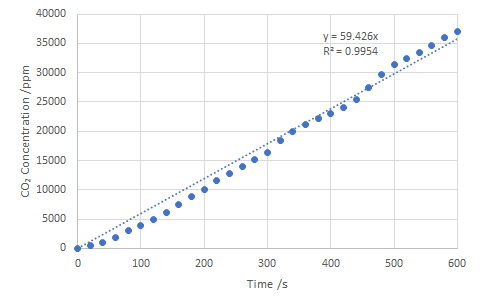
\includegraphics{figures/graph_01.png}
    \vspace*{-12pt}
    \caption{Carbon dioxide concentration plotted against time for 0.5\,\si{g} of glucose added}
    \label{fig:graph1}
    \renewcommand{\figurename}{Figure}
\end{figure}

The following table displays the equation for the line of best fit and $R^2$ values for each concentration:
\begin{table}[H]
\centering
\caption{Observations and concentrations for different masses of glucose added. Uncertainty for average slope was calculated using the half range method.}
\label{table:4}
\begin{tabularx}{\textwidth} {
    | >{\hsize=.26\hsize \linewidth=\hsize \raggedright\arraybackslash}X
    | >{\hsize=.27\hsize \linewidth=\hsize \raggedright\arraybackslash}X
    | >{\hsize=.27\hsize \linewidth=\hsize \raggedright\arraybackslash}X
    | >{\hsize=.2\hsize \linewidth=\hsize \raggedright\arraybackslash}X |}
    \hline
    \rowcolor[HTML]{CCCCCC} Glucose concentration /\si{M} & Line of best fit equation and $R^2$ for trial 1 & Line of best fit equation and $R^2$ for trial 2 & Average slope (initial reation velocity) /\si{ppm.s^{-1}} \\
    \hline
    $0.0056 \pm 0.0006$ & $y=35.324x, R^2=0.9962$ & $y=81.96x, R^2=0.9936$ & $59 \pm 20$ \\
    \hline
    $0.0139 \pm 0.0006$ & $y=59.095x, R^2=0.9805$ & $y=85.884x, R^2=0.9979$ & $72 \pm 10$ \\
    \hline
    $0.0278 \pm 0.0007$ & $y=59.426x, R^2=0.9954$ & $y=82.694x, R^2=0.9886$ & $71 \pm 10$ \\
    \hline
    $0.0555 \pm 0.0008$ & $y=36.929x, R^2=0.9789$ & $y=68.013x, R^2=0.9648$ & $52 \pm 20$ \\
    \hline
\end{tabularx}
\end{table}

With the processed data in tablex, reaction velocity can be plotted against glucose concentration to obtain the Michaelis Menten model. Doing a curve fit in excel reveals $V_{max} \approx -99$ and $K_2 \approx -99$

\section{Analysis}

\section{Evaluation}

\section{Conclusion}
Although the experiment did not match up perfectly with the theory, the results still made sense as a whole for a sufficient level of analysis. Evidently, this experiment models an extremely downscaled version of the many aspects involved in baking, thus presenting itself as more of a study into fermentation and enzyme kinetics rather than a practical guide to baking the best loaf of bread. In conclusion, the explanation of yeast producing carbon dioxide to cause bread to rise is widely accepted by many, but also an understatement, because it often unacknowledges the complex and fascinating chemistry involved behind the scenes.

\nocite{*}

\newpage

\printbibliography

\newpage

% TODO figure out why "appendices" are not preferred
\section{Appendices}

\subsection{Appendix A}

\subsection{Appendix B}

\subsection{Appendix C}

\subsection{Appendix D}

\subsection{Appendix E}

\end{document}}